\section{The WSN construction}
\begin{frame}{Block Ciphers}
    \centering
    \begin{tikzpicture}
    \begin{scope}
        \node (f0) at (-4,0) [minimum size=3cm,rounded corners=1ex,fill=black!80!white,draw] {{\sc \textcolor{white}{Enc}}};
        \node (m0) [above of=f0, node distance=2.25cm] {$p \in \set{0,1}^n$};
        \node (k0) [left of=f0, node distance=2.75cm] {$k \in \set{0,1}^n$};
        \node (c0) [below of=f0, node distance=2.25cm] {$c \in \set{0,1}^n$};
        \draw[-latex, thick] (m0) -- (f0);
        \draw[-latex, thick] (k0) -- (f0);
        \draw[-latex, thick] (f0) -- (c0);

        \node (title) [above of=m0, xshift=0pt, yshift=0pt, align=center] {Encrypt plaintext in blocks $p$ of $n$ bits,\\under a key of $n$ bits:};
    \end{scope}
    \visible<2->{%
    \begin{scope}
        \fill [fill=white, opacity=0.8, rounded corners=1ex] (0, 3.8) rectangle (4.5, -3.2);
        \node (xor-in) [right=150pt of m0, yshift=15pt] {};
        \node (diff-char) [below=-35pt of xor-in, xshift=-6pt] {\includegraphics[height=0.8\textheight]{data/spn}};

    \end{scope}
    }
    \end{tikzpicture}
    \visible<1->{%
        \note{%
        \begin{itemize}
            \item<1-> Block ciphers encrypt \emph{blocks} of $n$-bit inputs under an $n$-bit master key
            \item<1-> As a basic cryptographic primitive, we need special modes of operations,\\
                    if the data to be encrypted is not of exactly $n$-bit length.
            \item<1-> This we do not consider here, instead we want to look at how to build this black box.
        \end{itemize}
        }
    }
    \visible<2->{%
        \note{%
        \begin{itemize}
            \item Typicall approach is an SPN structure, where key-addition, S-box layer and\\
                  a linear layer are iterated over several rounds.
            \item Relatively well understood
            \item Good security arguments against known attacks
            \item There are some problems: differentials and linear hull effects
        \end{itemize}
        }
    }
\end{frame}

\begin{frame}{The WSN construction}
    \centering
    Published by \href{https://doi.org/10.1007/978-3-662-48800-3_18}{Tessaro at AsiaCrypt 2015} [\texttt{\href{https://ia.cr/2015/868}{ia.cr/2015/868}}].
    \begin{minipage}[t][90pt][t]{0.47\textwidth}
        \begin{block}{Overview round, iterated $r$ times\vpPp}
            \centering
            \vfill
            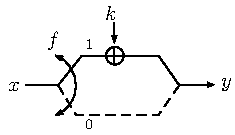
\includegraphics{data/wsn-schematic-1round}
            \vfill
        \end{block}
    \end{minipage}
    \hspace{5pt}
    \begin{minipage}[t][90pt][t]{0.47\textwidth}
        \begin{block}{Whitened Swap-Or-Not round function}
            \vspace*{-12.5pt}
            \begin{gather*}
                x, k \in \set{0,1}^n \quad\text{and}\quad f_{k} : \set{0,1}^n \to \set{0,1} \\
                y = \begin{cases*}
                    x + k & if $f_{k}(x) = 1$ \\
                    x     & if $f_{k}(x) = 0$
                    \end{cases*}
            \end{gather*}
        \end{block}
    \end{minipage}

    \visible<2->{%
    \vspace*{5pt}
    \begin{minipage}[t][60pt][t]{0.98\textwidth}
        \begin{block}{Security Proposition (informal)}
            \centering
            The WSN construction with $r = \Theta(n)$ rounds is
            \emph{Full Domain} secure.
            \vspace{3pt}
        \end{block}
    \end{minipage}
    }

    \only<1->{\note{\begin{itemize}
        \item Lets take a look at the WSN construction (simplified).
        \item Again, an iterated round function, where the input is fed into from the left.
        \item Next, a Boolean function decides if either the round key $k$ is xored onto the input, or nothing happens.
        \item The result is the updated state, respective the output of the round.
        \item In other words, $x$, and $k$ are both $n$-bit strings and $f$ is an $n$-bit Boolean function.
        \item The round output $y$ is either $x+k$ if $f_k(x) = 1$ or just $x$ in the other case.
        \item So why is this nice?
    \end{itemize}}}
    \only<2->{\note{\begin{itemize}
        \item Tessaro was able to show that this construction, when iterated over $\Theta(n)$ rounds, achieves \emph{Full Domain} security (what ever that means).
        \item One further property of $f$ which we need for decryption is that $x$ and $x+k$ maps to the same output.
    \end{itemize}}}
\end{frame}

\begin{frame}{An Implementation}
    \visible<2->{%
    \begin{minipage}{0.56\textwidth}
        \centering
        \begin{block}{Construction}
            \begin{itemize}
                \item $f_k(x) \coloneqq\ $?
                \item Key schedule?
                \item $\Theta(n)$ rounds?
            \end{itemize}
        \end{block}
        \vspace{5pt}
        Theoretical vs.\ practical constructions
    \end{minipage}
    \hfill
    \begin{minipage}{0.40\textwidth}
        \centering
        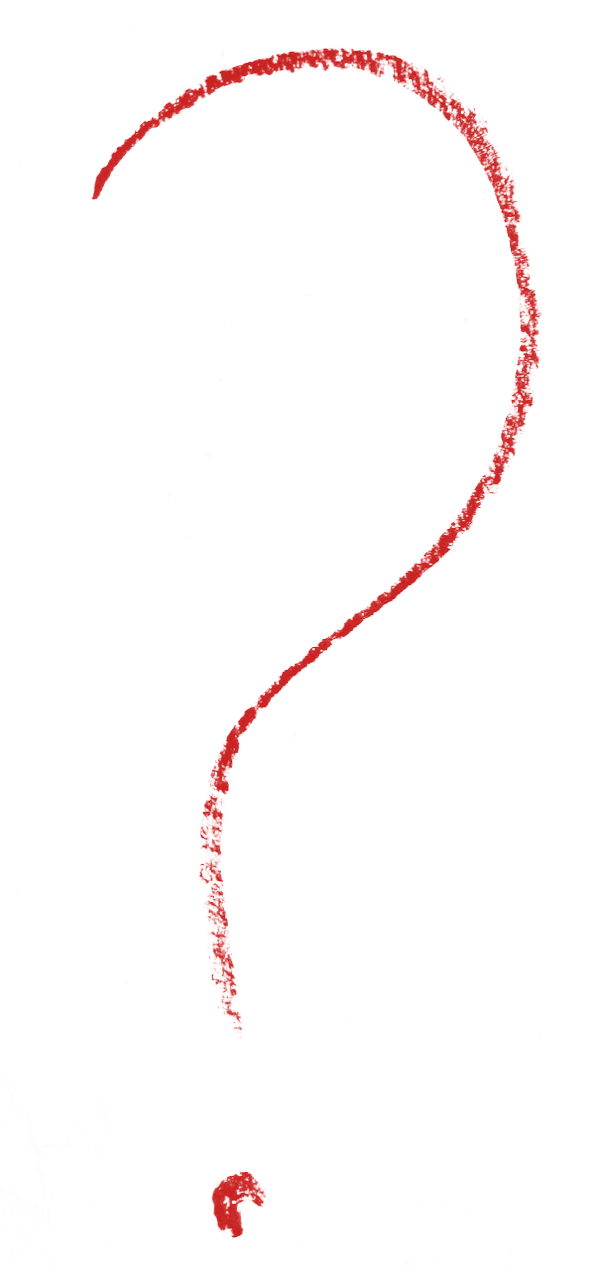
\includegraphics[height=0.6\textheight]{data/flickr/questionmark-alertred}
    \end{minipage}
    }
    \only<1->{\note{\begin{itemize}
        \item Sounds all very great.
        \item So from a practitioners point of view the natural next point is: lets implement it.
    \end{itemize}}}
    \only<2->{\note{\begin{itemize}
        \item But uggh\dots
        \item How does this Boolean function $f_k$ actually looks like?
        \item What about a key schedule? How do we derive the round keys?
        \item And how many are $\Theta(n)$ rounds?
    \end{itemize}
    \begin{itemize}
        \item So, from a theoretical point of view we have a nice construction.
        \item But from a practical point of view it is basically useless.
    \end{itemize}
    \begin{itemize}
        \item OK, let us fix this.
    \end{itemize}}
    }
\end{frame}

\section{Generic Analysis}
\begin{frame}{The WSN construction}{Encryption}
    \centering
    \begin{forest}
        %for tree={grow=east},
        [{\textcolor{green!90!blue}{$x$}},
        name=root,
        for children={visible on=<2->}
            [{$x$},
            for children={visible on=<3->}
                [{$x$},
                for children={visible on=<4->}
                    [{$x$}, name=left node]
                    [{$x + k_2$}]
                ]
                [{$x + k_1$},
                for children={visible on=<4->}
                    [{$x + k_1$}]
                    [{$x + k_1 + k_2$}]
                ]
            ]
            [{\textcolor{green!90!blue}{$x + k_0$}},
            edge={thick, green!90!blue},
            for children={visible on=<3->}
                [{\textcolor{green!90!blue}{$x + k_0$}},
                edge={thick, green!90!blue},
                for children={visible on=<4->}
                    [{$x + k_0$}]
                    [{\textcolor{green!90!blue}{$x + k_0 + k_2$}},
                    edge={thick, green!90!blue}
                    ]
                ]
                [{$x + k_0 + k_1$},
                for children={visible on=<4->}
                    [{$x + k_0 + k_1$}]
                    [{$x + k_0 + k_1 + k_2$}, name=right node]
                ]
            ]
        ]
        \node[above of=root, yshift=-15pt] {Input};
    \end{forest}

    \visible<4->{%
    %\vspace{-15pt}
    \begin{equation*}
        \text{Encryption:}\qquad
        E_{k}(x) \coloneqq x + \sum_{i=1}^{r} \lambda_i k_i = y
    \end{equation*}
    }

    \only<1->{\note{\begin{itemize}
        \item We can observe an interesting first property, when looking at the encryption procedure round by round
        \item Starting with the plaintext $x$\dots
    \end{itemize}}}
    \only<2->{\note{\begin{itemize}
        \item \dots in each round, we either add the round key $k_i$, \dots
    \end{itemize}}}
    \only<3->{\note{\begin{itemize}
        \item \dots or not.
    \end{itemize}}}
    \only<4->{\note{\begin{itemize}
        \item Thus we end up with a binary tree of possible states.
        \item Furthermore, the encryption can also be written as the plaintext plus the sum of some round keys, chosen by the $\lambda_i$'s here.
    \end{itemize}}}

\end{frame}

\begin{frame}{Generic Analysis}{On the number of rounds}
    \vspace{-20pt}
    \begin{minipage}[t][85pt][t]{0.47\textwidth}
        \begin{block}{Observation\vpPp}
            \begin{itemize}
                \item The ciphertext is the plaintext plus a subset of the round keys:
                    \begin{equation*}
                        y = x + \sum_{i=1}^{r} \lambda_i k_i
                    \end{equation*}
                \item For pairs $x_i, y_i$: $\Span \set{x_i + y_i} \subseteq \Span \set{k_j}$.
            \end{itemize}
            \vspace{2pt}
        \end{block}
    \end{minipage}
    \hfill
    \begin{minipage}[t][85pt][t]{0.47\textwidth}
        \visible<2->{%
        \begin{alertblock}{Distinguishing Attack for $r < n$ rounds\vpPp}
            \vspace{2pt}
            There is an $u \in \F_2^n \setminus \set{0}$, \st/ $\angles{u, x} = \angles{u, y}$ holds always:
            \begin{align*}
                        &\angles{u, y} = \angles{u, x + \sum \lambda_i k_i} \\
                        =\ &\angles{u, x} + \angles{u, \sum \lambda_i k_i} = \angles{u, x} + 0
                    \end{align*}
            for all $u \in \Span\set{k_1, \ldots, k_r}^\perp \neq \set{0}$
            \vspace{3pt}
        \end{alertblock}
        }
    \end{minipage}

    \vspace{50pt}

    \begin{minipage}{0.985\textwidth}
    \visible<3->{%
    \begin{exampleblock}{Rationale 1}
        Any instance must iterate at least n rounds; any set of n consecutive keys should be linearly indp.\vphantom{$\frac{1}{2}$}
    \end{exampleblock}
    }
    \end{minipage}
    \only<1->{\note{\begin{itemize}
        \item First observation: $\Span \set{x_i + y_i} \subseteq \Span \set{k_j}$
        \item Leads to a simple distinguishing attack, \emph{if number of rounds $r < n$}.
    \end{itemize}}}
    \only<2->{\note{\begin{itemize}
        \item It is easy to find a $u$, \st/ $\angles{u, y} = \angles{u, x} = 0$ for all $x, y = x, E(x)$.
        \item Simply use the bilinearity of the scalar product.
        \item Then any $u$ from the dual space spanned by the round keys fullfills the above equation.
        \item As long as there are less then $n$ round keys, this dual space has dimension greater or equal then one.
    \end{itemize}}}
    \only<3->{\note{\begin{itemize}
        \item A first design rational is thus\ldots
    \end{itemize}}}
\end{frame}

\begin{frame}{Generic Analysis}{On the Boolean functions $f$}
    \centering

    A bit out of the clear blue sky, but:

    \begin{exampleblock}{Rationale 2}
        For any instance, $f_{k}$ has to depend on all bits, and for any $\delta \in \F_2^n:\ \Pr\bracket{f_k(x) = f_k(x + \delta)} \approx \frac{1}{2}$.
    \end{exampleblock}

    \note{\begin{itemize}
        \item We also need this second rationale.
        \item Its not so easy explainable without going into more depth.
        \item So you have to believe me on this one.
        \item It basically says that for any input difference $\delta \neq k$:
              \begin{equation*}
                  \Pr\bracket{f_k(x) = f_k(x + \delta)} \approx \frac{1}{2}
              \end{equation*}
    \end{itemize}}
\end{frame}

\begin{frame}{A genus of the WSN family: \bison/}
    \centering
    \begin{exampleblock}{Rationale 1}
        Any instance must iterate at least n rounds; any set of n consecutive keys should be linearly indp.\vphantom{$\frac{1}{2}$}
    \end{exampleblock}
    \begin{exampleblock}{Rationale 2}
        For any instance, $f_{k}$ has to depend on all bits, and for any $\delta \in \F_2^n:\ \Pr\bracket{f_k(x) = f_k(x + \delta)} \approx \frac{1}{2}$.
    \end{exampleblock}
    \begin{block}{Generic properties of {\textbf{B}ent wh\textbf{I}tened \textbf{S}wap \textbf{O}r \textbf{N}ot} (\bison/)}
        \vspace{5pt}
        \begin{minipage}{0.51\textwidth}
        \begin{itemize}
            \item \only<1>{At least $n$ iterations of the round function}
                  \only<2>{\textcolor{alertred}{At least $n$ iterations of the round function}}
            \item Consecutive round keys linearly independent
        \end{itemize}
        \end{minipage}
        \begin{minipage}{0.44\textwidth}
        \begin{itemize}
            \item \only<1>{The round function depends on all bits}
                  \only<2>{\textcolor{alertred}{The round function depends on all bits}}
            \item $\forall \delta :\ \Pr\bracket{f_k(x) = f_k(x + \delta)} = \frac{1}{2}$ (\emph{bent})
        \end{itemize}
        \end{minipage}
        \vspace{5pt}
    \end{block}
    \visible<2->{%
        \vfill
        \begin{minipage}{0.47\textwidth}
            \centering
            \textcolor{alertred}{Rational 1 \& 2: WSN is \emph{slow} in practice!}
        \end{minipage}
        \hfill
        \begin{minipage}{0.47\textwidth}
            \centering
            The advantage?\\
            \Large
            Differential Cryptanalysis!
        \end{minipage}
        \vfill
    }
    \only<1->{\note{\begin{itemize}
        \item A quick recap and implications for any WSN instance.
        \item Rationale 2 basically tells us, we have to use \emph{bent} functions.
        \item Thats nice, as those functions are quite well understood and already well scrutinised.
        \item Also, this is the reason for the name: Bent Whitened Swap-Or-Not
        \item But, and thats not so nice\ldots
    \end{itemize}}}
    \only<2->{\note{\begin{itemize}
        \item $n$ iterations of a round function that depends on \emph{all} bits will be slow
        \item Let me repeat this (Reviewer 2 argued that we should optimise more):\\
              No matter how good we will optimise this: \emph{it will be slow}
        \item For example, assume you can do one round in one clock cycle,\\
              this is still an order of magnitude slower than AES\@.
        \item So, why should we care about any instance?
        \item All hope is not lost, let's have a look at differential cryptanalysis!
    \end{itemize}}}
\end{frame}

\section{Differential Analysis}
\begin{frame}{Differential Cryptanalysis}{Primer}
    \centering
    \begin{tikzpicture}
    \tikzfading[name=fade out, inner color=transparent!0, outer color=transparent!100]
    \only<1>{%
        \node (f0) at (0,0) [minimum size=3cm, minimum height=4cm, rounded corners=1ex,fill=black!80!white,draw] {{\sc \textcolor{white}{Enc}}};
        \node (m0) [above=10pt of f0.north] {$p$};
        \node (k0) [left=10pt of f0.west] {$k$};
        \node (c0) [below=10pt of f0.south] {$c$\vphantom{$^\prime$}};
        \draw[-latex, thick] (m0) -- (f0);
        \draw[-latex, thick] (k0) -- (f0);
        \draw[-latex, thick] (f0) -- (c0);

        \node (f1) at (5cm, 0) [minimum size=3cm, minimum height=4cm, rounded corners=1ex,fill=black!80!white,draw] {{\sc \textcolor{white}{Enc}}};
        \node (m1) [above=10pt of f1.north] {$p^\prime$};
        \node (k1) [right=10pt of f1.east] {$k$};
        \node (c1) [below=10pt of f1.south] {$c^\prime$};
        \draw[-latex, thick] (m1) -- (f1);
        \draw[-latex, thick] (k1) -- (f1);
        \draw[-latex, thick] (f1) -- (c1);

        \node (xor-in) [right=57.5pt of m0] {$\oplus$};
        \node (xor-out) [right=57.5pt of c0] {$\oplus$};
        \node (delta-in) [right=80pt of m1] {$= \textcolor{alertred}{\alpha}$};
        \node (delta-out) [right=80pt of c1] {$= \textcolor{alertred}{\beta}$};
        \draw[-latex, thick, dashed, color=alertred] (delta-in)+(4.5pt, -5pt) -- +(4.5pt, -145pt);
    }
    \only<2->{%
        \begin{scope}[opacity=0.2]
        \node (f0) at (0,0) [minimum size=3cm, minimum height=4cm, rounded corners=1ex,fill=white,draw] {{\sc Enc}};
        \node (m0) [above=10pt of f0.north] {$p$};
        \node (k0) [left=10pt of f0.west] {$k$};
        \node (c0) [below=10pt of f0.south] {$c$\vphantom{$^\prime$}};
        \draw[-latex, thick] (m0) -- (f0);
        \draw[-latex, thick] (k0) -- (f0);
        \draw[-latex, thick] (f0) -- (c0);

        \node (f1) at (5cm,0) [minimum size=3cm, minimum height=4cm, rounded corners=1ex,fill=white,draw] {{\sc Enc}};
        \node (m1) [above=10pt of f1.north] {$p^\prime$};
        \node (k1) [right=10pt of f1.east] {$k$};
        \node (c1) [below=10pt of f1.south] {$c^\prime$};
        \draw[-latex, thick] (m1) -- (f1);
        \draw[-latex, thick] (k1) -- (f1);
        \draw[-latex, thick] (f1) -- (c1);

        \node (xor-in) [right=57.5pt of m0] {$\oplus$};
        \node (xor-out) [right=57.5pt of c0] {$\oplus$};
        \node (delta-in) [right=80pt of m1] {$= \textcolor{alertred}{\alpha}$};
        \node (delta-out) [right=80pt of c1] {$= \textcolor{alertred}{\beta}$};
        \draw[-latex, thick, dashed, color=alertred] (delta-in)+(4.5pt, -5pt) -- +(4.5pt, -145pt);
        \end{scope}
    }

    \visible<2->{%
        \fill [fill=white, opacity=0.8, rounded corners=1ex] (-1.75, 3.4) rectangle (8.25, -3.4);
    }

    \visible<2>{%
        \node (diff-char) [below=-22pt of xor-in, xshift=-50pt, yshift=11pt] {\includegraphics[height=0.8\textheight]{data/differential1}};
    }
    \visible<2->{%
        \node (prob-diff1) [right=10pt of diff-char, yshift=70pt, align=center] {%
            $\begin{aligned}
                \Prob\bracket{\alpha \stackrel{E_k}{\to} \beta} =\ ?
            \end{aligned}$
        };
    }

    \visible<3>{%
        \node (diff-char) [below=-22pt of xor-in, xshift=-50pt, yshift=11pt] {\includegraphics[height=0.8\textheight]{data/differential-characteristic}};
    }
    \visible<3->{%
        \node (prob-char) [right=10pt of diff-char, yshift=0pt, align=center] {%
            $\begin{aligned}
                p_\theta &= \Prob\bracket{\theta_0 \stackrel{R}{\to} \theta_1 \stackrel{R}{\to} \cdots \stackrel{R}{\to} \theta_r} \\
                         &= \prod_{i=0}^{r-1} \Prob\bracket{\theta_i \stackrel{R}{\to} \theta_{i+1}}
            \end{aligned}$
        };
    }

    \visible<4->{%
        \node (diff) [below=-22pt of xor-in, xshift=-50pt, yshift=11pt] {\includegraphics[height=0.8\textheight]{data/differential2}};
    }
    \visible<4->{%
        \node (prob-diff2) [right=10pt of diff, yshift=-70pt, align=center] {%
            $\begin{aligned}
                \Prob\bracket{\alpha \stackrel{E_k}{\to} \beta} = \sum_{\theta} p_\theta
            \end{aligned}$
        };
    }
    \end{tikzpicture}
    \only<1->{\note{\begin{itemize}
        \item For differential cryptanalysis, interested in propagation of input difference $\alpha$ to output difference $\beta$.
        \item Doing this in general at this abstraction level is a very hard problem.
    \end{itemize}}}
    \only<2->{\note{\begin{itemize}
        \item To say anything, we usually look for single so called \emph{trails} through the inner building blocks.
    \end{itemize}}}
    \only<3->{\note{\begin{itemize}
        \item Now, computing the probability of one such trail is actually doable.
        \item But, trails can go several alternative ways through non-linear parts, thus we have to cope with a branching effect\ldots
    \end{itemize}}}
    \only<4->{\note{\begin{itemize}
        \item And eventually, several of these trails cluster in a so called \emph{differential}.
        \item While in this example it is still feasible, computing the \emph{exact} probability in a real cipher is not.
        \item We thus have to restrain on bounding or approximating this probability.
        \item In the end, tight bounds for differentials over several rounds remain an open (but important!) problem.
    \end{itemize}
    \begin{itemize}
        \item For \bison/ our aim is to give exactly this: a tight bound for any differential over several rounds.
    \end{itemize}}}
\end{frame}

\begin{frame}{Differential Cryptanalysis}{One round}
    \vspace{-30pt}
    \begin{columns}
        \begin{column}{0.58\textwidth}
            \centering
            \vspace{30pt}
            \begin{block}{Proposition}
                %\centering
                For one round of \bison/
                the probabilities are:
                \begin{equation*}
                    \Prob\bracket{\alpha \to \beta} = \begin{cases*}
                        1           & if $\alpha = \beta = k$ or $\alpha = \beta = 0$\\
                        \frac{1}{2} & else if $\beta \in \set{\alpha, \alpha + k}$\\
                        0           & else
                    \end{cases*}
                \end{equation*}
            \end{block}
        \end{column}
        \begin{column}{0.40\textwidth}
            \vspace{40pt}
            \centering
            \vfill
            \visible<2->{%
                \begin{block}{Possible differences}
                    \vspace{-20pt}
                    \begin{alignat*}{5}
                                &x   &          &+ \hphantom{(} f_k(x)\ &                                \cdot &k \\
                        \oplus\ &x\  &+\ \alpha &                       &+\ f_k(x + \alpha) \hphantom{)} \cdot &k \\
                        =\      &    &\alpha\   &+ (f_k(x)\             &+\ f_k(x + \alpha))             \cdot &k
                    \end{alignat*}
                    \vspace{-17pt}
                \end{block}
                \begin{block}{Properties of $f_{k}$\vpPp}
                    \vspace{-5pt}
                    \begin{equation}
                        f_k(x) = f_k(x + k)
                    \end{equation}
                    \visible<3->{%
                    \vspace{-10pt}
                    \begin{equation}
                        \Pr\bracket{f_k(x) = f_k(x + \alpha)} = \frac{1}{2}
                    \end{equation}
                }
                    %\vspace{-10pt}
                \end{block}
            }
        \end{column}
    \end{columns}
    \only<1->{\note{\begin{itemize}
        \item We start by understanding the differential one round behaviour.
        \item For the three possible cases, let us look at what differences are actually possible.
    \end{itemize}}}
    \only<2->{\note{\begin{itemize}
        \item Remember that one round computes the output as $x + f_k(x) \cdot k$.
        \item With the input difference $\alpha$ we get as possible output differences $\beta \in \set{0, \alpha, k, \alpha + k}$.
        \item For decryption we need that $x$ and $x+k$ are mapped to the same value by $f_k$
        \item Thus, $\beta = \alpha$ with probability one, if and only if $\alpha = k$ or $\alpha = 0$
        \item If $\beta$ is not one of the above four values, such an input/output pair cannot occur,\\
              thus the probability is zero.
    \end{itemize}}}
    \only<3->{\note{\begin{itemize}
        \item For the last case, remember that for any input difference, we required\\
              that $f_k$ collides with probability one half.
    \end{itemize}}}
\end{frame}

\begin{frame}{Differential Cryptanalysis}{More rounds}
    Example differences over $r = 3$ rounds ($\alpha = k_1 + k_2$):\\
    \begin{center}
    \only<1>{%
    \begin{forest}
        [{$\alpha$}
            [{$\alpha$},
            edge label={node[midway,left,yshift=2mm,font=\scriptsize] {$\frac{1}{2}$}}
                [{$\alpha$}
                    [{$\alpha$}]
                    [{$\alpha + k_3$}]
                ]
                [{$\alpha + k_2$}
                    [{$\alpha + k_2$}]
                    [{$\alpha + k_2 + k_3$}]
                ]
            ]
            [{$\alpha + k_1$},
            edge label={node[midway,right,yshift=2mm,font=\scriptsize] {$\frac{1}{2}$}}
                [{$\alpha + k_1$},
                edge={thick},
                edge label={node[midway, left, yshift=2mm, font=\scriptsize] {$1$}}
                    [{$\alpha + k_1$}]
                    [{$\alpha + k_1 + k_3$}]
                ]
                [{$\alpha + k_1 + k_2$},
                edge={dotted, thick},
                edge label={node[midway, right, yshift=2mm, font=\scriptsize] {$0$}}
                    [{$\alpha + k_1 + k_2$}]
                    [{$\alpha + k_1 + k_2 + k_3$}]
                ]
            ]
        ]
    \end{forest}}\only<2>{%
    \begin{forest}
        [\textcolor{alertred}{$\alpha$}
            [\textcolor{alertred}{$\alpha$},
            edge={color=alertred, thick},
            edge label={node[midway,left,yshift=2mm,font=\scriptsize] {$\frac{1}{2}$}}
                [{$\alpha$}
                    [{$\alpha$}]
                    [{$\alpha + k_3$}]
                ]
                [\textcolor{alertred}{$\alpha + k_2$},
                edge={color=alertred, thick}
                    [\textcolor{alertred}{$\alpha + k_2$},
                    edge={color=alertred, thick}]
                    [{$\alpha + k_2 + k_3$}]
                ]
            ]
            [{$\alpha + k_1$},
            edge label={node[midway,right,yshift=2mm,font=\scriptsize] {$\frac{1}{2}$}}
                [{$\alpha + k_1$},
                edge={thick},
                edge label={node[midway, left, yshift=2mm, font=\scriptsize] {$1$}}
                    [{$\alpha + k_1$}]
                    [{$\alpha + k_1 + k_3$}]
                ]
                [{$\alpha + k_1 + k_2$},
                edge={dotted, thick},
                edge label={node[midway, right, yshift=2mm, font=\scriptsize] {$0$}}
                    [{$\alpha + k_1 + k_2$}]
                    [{$\alpha + k_1 + k_2 + k_3$}]
                ]
            ]
        ]
    \end{forest}}
    %\vspace{10pt}

    \visible<2->{%
        \begin{theorem}[Differentials in \bison/]
            \vspace{5pt}
            Let $\alpha$, $\beta \in \F_2^n$.
            Then the probability for the differential $\alpha \to \beta$ is
            $\displaystyle \Prob\bracket{\alpha \to \beta} = \sum_\theta p_\theta = p_{(\alpha, \theta_1, \ldots, \theta_{r-1}, \beta)}$.
        \end{theorem}
    }
    \end{center}
    \only<1->{\note{\begin{itemize}
        \item When we look at more rounds, we can depict these cases again in this tree structure.
        \item Starting with the input difference $\alpha$, assume it is different from the first round key $k_0$ and nonzero.
        \item After one round the two differences $\alpha$ and $\alpha + k_0$ occur with equal probability one half.
        \item As long as the intermediate difference is different from the next round key and nonzero,\\
              this argument iterates.
        \item At the point where the difference equals the next round key,\\
              these two choices collide into a deterministic propagation with probability one,\\
              where the round key is not added to the difference.
    \end{itemize}}}
    \only<2->{\note{\begin{itemize}
        \item Regarding differentials, the important observation is:
        \item For any input/output pair $(\alpha, \beta)$, there is only one path.
        \item In other words: no branching occurs and the differential consists of a single trail only.
    \end{itemize}}}
\end{frame}

\section{The concrete Instance}
\begin{frame}{BISON}
    \centering
    \begin{minipage}{0.63\textwidth}
    \centering
    \begin{block}{A concrete species}
        \centering
        \vspace{2pt}
        
\includegraphics[height=0.7\textheight]{data/bison-logo}
    \end{block}
    \end{minipage}
    \only<1->{\note{\begin{itemize}
        \item Up to now we do not have specified much more then the initial WSN construction had.
        \item For a concrete implementation, we still need to define
              \begin{itemize}
                  \item Number of rounds
                  \item Key Schedule
                  \item Boolean function $f_k$
              \end{itemize}
        \item So let us look at a concrete \bison/ species
        \item In particular, we discuss how to tackle Rationales 1 and 2.
    \end{itemize}}}
\end{frame}

\begin{frame}{Addressing Rationale 1}{The Key Schedule}
    \vspace{-60pt}
    \begin{minipage}{0.985\textwidth}
    \begin{exampleblock}{Rationale 1}
        Any instance must iterate at least n rounds; any set of n consecutive keys should be linearly indp.\vphantom{$\frac{1}{2}$}
    \end{exampleblock}
    \end{minipage}

    \begin{minipage}[t][85pt][t]{0.47\textwidth}
        \begin{block}{Design Decisions}
            \begin{itemize}
                \item Choose number of rounds as $3 \cdot n$\\[5pt]
                \item Round keys derived from the state of LFSRs\\[5pt]
                \item Add round constants $c_i$ to $w_i$ round keys
            \end{itemize}
        \end{block}
    \end{minipage}
    \hfill
    \begin{minipage}[t][85pt][t]{0.47\textwidth}
        \begin{block}{Implications}
            \begin{itemize}
                \item Clocking an LFSR is cheap
                \item For an LFSR with irreducible feedback polynomial of degree $n$, every $n$ consecutive states are linearly independent
                \item Round constants avoid structural weaknesses
            \end{itemize}
        \end{block}
    \end{minipage}
    \only<1->{\note{\begin{itemize}
        \item Due to analysis of the alg.~deg., we chose $3n$ rounds, see last slide.
        \item Deriving round keys from the states of LFSRs is efficiently implementable and\\
              fullfils our requirements for linear independent round keys.
        \item For those of you how attended Gregors talk at FSE:
              \begin{itemize}
                  \item While generating test vectors for the implementation we again noted some\\
                        unwanted symmetries for encryptions with low hamming weight.
                  \item Thus we added round constants, to avoid these structural weaknesses.
                  \item (Sorry for fixing another cipher)
              \end{itemize}
    \end{itemize}}}
\end{frame}

\begin{frame}{Addressing Rationale 2}{The Round Function}
    \vspace{-60pt}
    \begin{minipage}{0.985\textwidth}
    \begin{exampleblock}{Rationale 2}
        For any instance, the $f_{k}$ should depend on all bits, and for any $\delta \in \F_2^n:\ \Pr\bracket{f_k(x) = f_k(x + \delta)} \approx \frac{1}{2}$.
    \end{exampleblock}
    \end{minipage}

    \begin{minipage}[t][85pt][t]{0.47\textwidth}
        \begin{block}{Design Decisions}
            \begin{itemize}
                \item Choose $f_k : \F_2^n \to \F_2$ \st/
                      \begin{equation*}
                          \delta \in \F_2^n:\ \Pr\bracket{f_k(x) = f_k(x + \delta)} = \frac{1}{2},
                      \end{equation*}
                      that is, $f_k$ is a bent function.
                \item Choose the simplest bent function known:
                    \begin{equation*}
                        f_k(x, y) \coloneqq \angles{x, y}
                    \end{equation*}
            \end{itemize}
        \end{block}
    \end{minipage}
    \hfill
    \begin{minipage}[t][85pt][t]{0.47\textwidth}
        \begin{block}{Implications}
            \begin{itemize}
                \item Bent functions well studied\\[5pt]
                \item Bent functions only exists for even $n$\\[5pt]
                \item Instance not possible for every block length $n$
            \end{itemize}
        \end{block}
    \end{minipage}
    \only<1->{\note{\begin{itemize}
        \item Just chose the simplest bent function, the scalar product.
        \item This is also efficiently implementable.
    \end{itemize}
    \begin{itemize}
        \item But, another drawback:
        \item Bent functions exists only for even $n$.
        \item Thus \bison/ cannot be instantiated for every block length $n$.
        \item In particular, due to reasons not covered here, we can actually\\
              only instantiate it for \emph{odd} block lengths.
    \end{itemize}}}
\end{frame}

\begin{frame}{An Implementation}
    \only<1>{%
    \begin{minipage}{0.47\textwidth}
        \centering
        \vspace*{-40pt}
        \begin{block}{Construction}
            \begin{itemize}
                \item \only<1>{$f_k(x) \coloneqq\ $?}\only<2->{$f_k(x, y) \coloneqq\ \angles{x, y}$}
                \item Key schedule\only<1>{?}\only<2->{: LFSRs.}
                \item \only<1>{$\Theta(n)$ rounds?}\only<2->{$\Theta(n) = 3n$ rounds}
            \end{itemize}
        \end{block}
    \end{minipage}
    \hfill
    \begin{minipage}{0.50\textwidth}
        \centering
        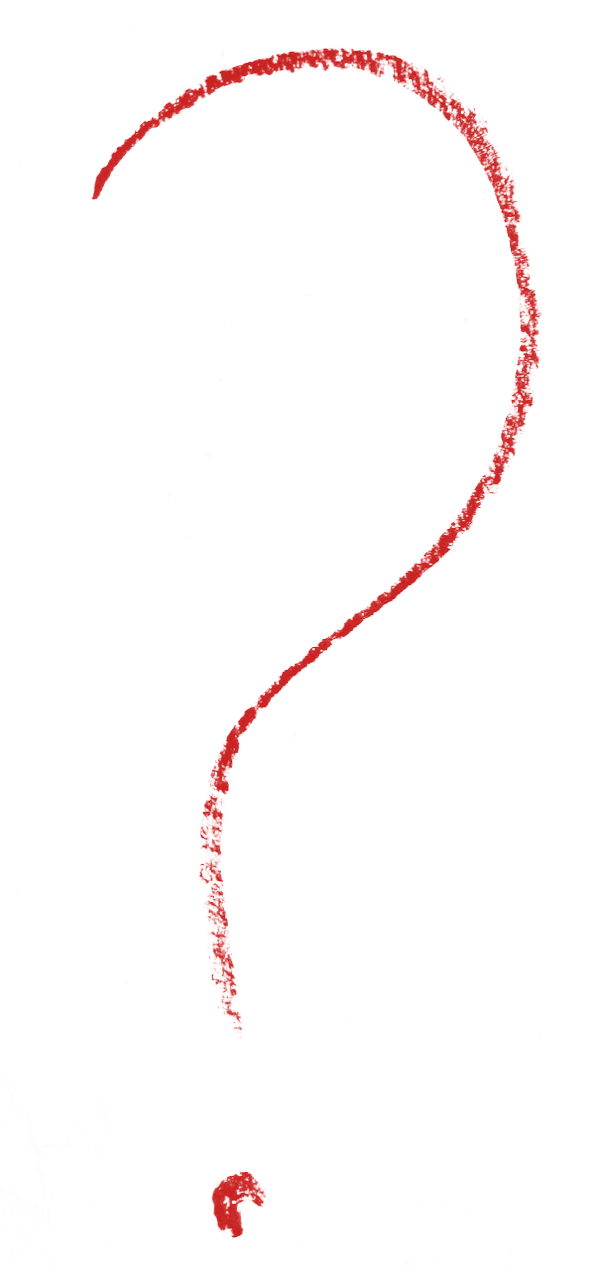
\includegraphics[height=0.6\textheight]{data/flickr/questionmark-alertred}
    \end{minipage}
    }
    \only<2->{
    \begin{minipage}{0.47\textwidth}
        \centering
        \begin{block}{Construction}
            \begin{itemize}
                \item $f_k(x, y) \coloneqq\ \angles{x, y}$
                \item Key schedule: LFSRs.
                \item $\Theta(n) = 3n$ rounds.
            \end{itemize}
        \end{block}
    \end{minipage}
    \vspace*{20pt}
    \hfill
    \visible<3->{%
        \begin{minipage}{0.47\textwidth}
            \centering
            \sisetup{%
                group-digits = integer,
                group-separator = {\,},
                group-minimum-digits = 4,
                table-text-alignment = center,
                table-number-alignment = center,
                table-figures-integer = 4,
                table-figures-decimal = 2,
            }
            \tabcolsep=5pt
            \begin{tabular}{ccS}
                \toprule
                Cipher    & Block size & {Cycles/Byte} \\
                            &    (bit)   &    {mean}     \\
                \midrule
                AES$^{*}$ &     128    &       0.65    \\
                \bison/$^{\dag}$ &     129    &    3064.08    \\
                \bottomrule
            \end{tabular}
        \end{minipage}
    }

    \visible<3->{%
        {\footnotesize
        $^{*}$~AES-128 on Skylake Intel\textregistered{} Core i7-7800X @ 3.5GHz, see Daemen et al.~[\href{https://tosc.iacr.org/article/view/7359}{The design of Xoodoo and Xoofff}, Table~5].
        $^{\dag}$~\bison/ on CoffeeLake Intel\textregistered{} Core i7-8700 @ 3.7 GHz.
        }
    }
    }
    \only<1->{\note{\begin{itemize}
        \item Coming back to our initial question.
        \item And basically only for the sake of completeness, as we already saw this is going to be slow.
    \end{itemize}}}
    \only<2->{\note{\begin{itemize}
        \item We have specified everything, so let's benchmark against AES (what else).
    \end{itemize}}}
    \only<3->{\note{\begin{itemize}
        \item OK, told you so, \bison/ is like 4\,700 times slower than AES\@.
        \item Or: more than three orders of magnitude.
        \item Optimising this will not help enough.
    \end{itemize}}}
\end{frame}

\section{Further Analysis}
\begin{frame}{Further Cryptanalysis}
    \vspace*{-15pt}
    \begin{minipage}[t][70pt][t]{0.47\textwidth}
        \begin{block}{Linear Cryptanalysis\vpPp}
            For $r \geqslant n$ rounds, the correlation of any non-trivial linear trail for \bison/ is upper bounded by $2^{-\frac{n+1}{2}}$.
        \end{block}
    \end{minipage}
    \hfill
    \begin{minipage}[t][70pt][t]{0.47\textwidth}
        \begin{block}{Invariant Attacks\vpPp}
            For $r \geqslant n$ rounds, neither invariant subspaces nor nonlinear invariant attacks do exist for \bison/.
            \vspace{3pt}
        \end{block}
    \end{minipage}

    \begin{minipage}[t][70pt][t]{0.47\textwidth}
        \begin{block}{Zero Correlation\vpPp}
            For $r > 2n-2$ rounds, \bison/ does not exhibit any zero correlation linear hulls.
        \end{block}
    \end{minipage}
    \hfill
    \begin{minipage}[t][70pt][t]{0.47\textwidth}
        \begin{block}{Impossible Differentials\vpPp}
            For $r > n$ rounds, there are no impossible differentials for \bison/.
            \vspace{2pt}
        \end{block}
    \end{minipage}

    \vspace*{-12.5pt}
    \begin{minipage}[t][30pt][t]{0.985\textwidth}
        \begin{block}{Algebraic Degree and Division Property\vpPp}
            Algebraic degree grows \emph{linearly}.
            Conservative estimate: for $r \geqslant 3n$ rounds, no attack possible.
        \end{block}
    \end{minipage}

    \only<1->{\note{\begin{itemize}
        \item We did more cryptanalysis, but our results are more of the \enquote{classical} kind.
        \item For linear cryptanalysis, we bound the correlation of any non-trivial trail.
        \item Current known security arguments for resistance against invariant attacks apply.
        \item Zero correlation and impossible differentials do not exist for $2n$ rounds or more.
        \item Best attacks seem to exploit the algebraic degree.
        \item We show that it grows only linearly -- which is especially bad in comparison to SPN ciphers.
        \item The result on the algebraic degree also applies to NLFSRs or maximally unbalanced Feistel networks.
        \item Conservative estimation: might work for more than $2n$ rounds, but not for $3n$ or more.
    \end{itemize}}}
\end{frame}

\begin{frame}{Conclusion/Questions}{Thank you for your attention!}
    \vspace{-25pt}
    \begin{minipage}[t][85pt][t]{0.47\textwidth}
        \begin{block}{\bison/\vpPp}
            \begin{itemize}
                \item A first instance of the WSN construction
                \item Good results for differential cryptanalysis
            \end{itemize}
        \end{block}
    \end{minipage}
    \hfill
    \begin{minipage}[t][85pt][t]{0.47\textwidth}
        \begin{block}{Open Problems}
            \begin{itemize}
                \item Construction for linear cryptanalysis?
                \item Similar args.\ for Unbalanced Feistel?
            \end{itemize}
        \end{block}
    \end{minipage}

    \vspace{30pt}

    \begin{tikzpicture}[overlay]
        \node (thanks) at (4,0){};
        \draw[rotate=-7,line width=1.5pt,saphierblau,fill=gray!10]
             ($(thanks)-(1.5,.35)$) rectangle ($(thanks)+(1.5,.35)$)
             node[rotate=-7] at (thanks) {\textcolor{saphierblau}{\textbf{Thank you!}}};

        \node[right=100pt of thanks](questions){};
        \draw[rotate=3,line width=1.5pt,saphierblau,fill=gray!10]
             ($(questions)-(1.15,.35)$) rectangle ($(questions)+(1.15,.35)$)
             node[rotate=3] at (questions) {\textcolor{saphierblau}{\textbf{Questions?}}};

        \node[right=100pt of questions](eprint){};
        \draw[rotate=14,line width=1.5pt,saphierblau,fill=gray!10]
             ($(eprint)-(1.15,.35)$) rectangle ($(eprint)+(1.15,.35)$)
             node[rotate=14] at (eprint) {\textcolor{saphierblau}{\textcolor{gelbgruen}{\textbf{\href{https://ia.cr/2018/1011}{2018/1011}}}}};
    \end{tikzpicture}
\end{frame}

%\begin{frame}[allowframebreaks]{References}
%    %\begingroup
%    %    \scriptsize Title Image: \href{https://www.flickr.com/photos/bluetrailphoto/11095367173/in/photolist-hUsE72-7X4eFa-qd7u6B-eTa8pd-hiDwGF-cSTY2d-cSU6Ky-eSXJJt-cSTXLq-cSTUhq-arJDEr-cLkoTm-QWsSn3-6rEB3f-qAcyWm-r9yN4b-8Rh3wU-8msPC1-8VN8Qb-5Nyggn-bjUxdV-ent85f-DnwchP-cp6bmJ-wPFFSv-NhRU6s-cp69Kq-Nm4z1F-QnDuHm-HJcDrV-rEdDTc-MPZXa9-6bRMU6-KcegAy-aQCqMx-cp6d4L-X1c1Ym-aohLov-SSV7w-STFfT-atKAhj-qZXa1M-aecFP9-iRFVou-SSUb7-cp6dzu-cxr1qG-eJVbbv-oMb4qu-251se6T}{Blue Trail Photography: \enquote{Lords of the Plains (b\&w)}, \emph{flickr}}\\[1em]
%    %\endgroup
%    %\begingroup
%    %    \scriptsize Questionmark Image: \emph{flickr}\\[1em]
%    %\endgroup
%    \tiny
%    \printbibliography{}
%\end{frame}

\begin{frame}[plain]
    \centering
    \Huge
    \vspace{-1\baselineskip}
    Details
\end{frame}

\section{Specification}
\begin{frame}{\bison/}{Round Function}
    \vspace{-45pt}
    \begin{minipage}[t][150pt][t]{0.985\textwidth}
        \begin{block}{BISON's round function\vpPp}
            \centering
            \vspace{0.5\baselineskip}
            For round keys $k_i\in \F_2^n$ and $w_i\in \F_2^{n-1}$ the round function computes
            \begin{equation*}
                R_{k_i, w_i}(x) \coloneqq x + f_{b(i)} \parens{w_i + \Phi_{k_i}\parens{x}} \cdot k_i.
            \end{equation*}
            \flushleft
            where
            \begin{itemize}
                \item $\Phi_{k_i}$ and $f_{b(i)}$ are defined as
            \end{itemize}
            \vspace{-10pt}
            \begin{columns}
                \begin{column}{0.49\textwidth}
                    \begin{align*}
                        \Phi_k(x) : \F_2^n &\to \F_2^{n-1} \\
                        \Phi_k(x) &\coloneqq (x + x[i(k)] \cdot k)[j]_{\tower{1 \leqslant j \leqslant n}{j \neq i(k)}}
                    \end{align*}
                \end{column}
                \begin{column}{0.49\textwidth}
                    \begin{align*}
                        f_{b(i)} : \F_2^{\frac{n-1}{2}}\times \F_2^{\frac{n-1}{2}} &\to \F_2 \\
                        f_{b(i)}(x,y) &\coloneqq \angles{x,y} + b(i),
                    \end{align*}
                \end{column}
            \end{columns}
            \begin{itemize}
                \item and $b(i)$ is $0$ if $i \leqslant \frac{r}{2}$ and $1$ else.
            \end{itemize}
            \vspace{-0.25\baselineskip}
        \end{block}
    \end{minipage}
\end{frame}

\begin{frame}{\bison/}{Key Schedule\vpPp}
    \vspace{-45pt}
    \begin{minipage}[t][150pt][t]{0.985\textwidth}
        \begin{block}{BISON's key schedule}
            \vspace{0.5\baselineskip}
            Given
            \begin{itemize}
                \item primitive $p_k$, $p_w \in \F_2[x]$ with degrees $n$, $n-1$ and companion matrices $C_k$, $C_w$.
                \item master key $K = (k, w) \in \parens{\F_2^n \times \F_2^{n-1}} \setminus \set{0,0}$
            \end{itemize}
            The $i$th round keys are computed by
            \begin{align*}
                \ks_i : \F_2^n \times \F_2^{n-1} &\to \F_2^n \times \F_2^{n-1} \\
                \ks_i(k, w) &\coloneqq (k_i, c_i + w_i)
            \end{align*}
            where \begin{equation*}
                    k_i = \parens{C_k}^i k, \qquad
                    c_i = \parens{C_w}^{-i} e_1, \qquad
                    w_i = \parens{C_w}^i w.
                \end{equation*}
        \end{block}
    \end{minipage}
\end{frame}
